\chapter{Введение}\label{introduction}

\section{О книге}

Начни изучать Эрланг во имя добра!
Чтение этого руководства, скорее всего, будет одним из твоих первых шагов в изучении Erlang, поэтому скажу о нём пару слов.

\begin{wrapfigure}{l}{0.3\linewidth}
    
\includegraphics[width=1\linewidth]{erlang.png}
\end{wrapfigure}

Во\--первых, идея написать это обучающее руководство появилась у меня после того, как я прочитал \href{http://learnyouahaskell.com}{Изучай Haskell во имя добра!} Miran Lipova\v{c}a.
Мне показалось, что ему удалось представить язык в привлекательном свете, и сделать процесс обучения приятным.
Я уже был знаком с Мираном, поэтому поинтересовался, как он относится к тому, что я напишу версию его книги, посвящённую Erlang.
Идея пришлась ему по душе, так как он и сам интересовался Erlang.

Всё это привело к тому, что я теперь печатаю эти слова.
Конечно, были и другие источники мотивации: я считаю что <<порог вхождения>> в язык довольно высок (в web маловато документации и, скорее всего, придётся покупать книги).
Поэтому я подумал, что сообществу пригодится руководство похожее на LYAH.
Ещё я заметил, что люди приписывали Erlang слишком много или слишком мало достоинств, основываясь при этом на поверхностных суждениях.
Есть люди, которые абсолютно уверены, что Erlang это просто разрекламированная пустышка.
Даже если бы я хотел их убедить в обратном, знаю, что они вряд ли прочитают эти строки.

Эта книга даёт возможность изучить Erlang тем, кто имеет базовые знания о программировании на императивных языках (таких как C/C++, Java, Python, Ruby и т.д.) и имеет или не имеет представление о функциональном программировании (Haskell, Scala, Erlang, Clojure, OCaml\ldots)
Также я хочу, чтобы эта книга честно рассказывала об Erlang, правдиво освещая слабые и сильные стороны языка.

\section{Так что же такое Erlang?}
Во\--первых, Erlang это функциональный язык программирования.
Если вам приходилось когда\--либо работать с императивными языками, то вы нормально относитесь к выражениям вроде \ops{i++;} в функциональном программировании такие выражения не разрешаются.
Более того, изменять значение любой переменной строго запрещено!
Сначала это может прозвучать странно, но если вы припомните уроки математики, то на них всё так и объясняли:\\ 
y = 2\\ 
x = y + 3\\ 
x = 2 + 3\\ 
x = 5\\ 
Если бы я добавил:\\ 
x = 5 + 1\\ 
x = x\\ 
$\therefore 5 = 6$\\ 

То привёл бы вас в замешательство.
В функциональном программировании принято так: если я говорю, что x это 5, то, согласно логике, я не могу заявить, что x также и 6!
Было бы нечестно.
Поэтому функции с одинаковыми параметрами всегда должны возвращать тот же результат:\\  
x = add\_two\_to(3) = 5\\ 
$\therefore x = 5$
 
Функции, которые  всегда возвращают одинаковый результат для тех же параметров, называются чистыми.
Именно поэтому мы можем заменить  \ops{add\_two\_to(3)} на 5, потому что результат операции \ops{3+2} будет всегда равен 5.
Это означает, что мы можем компоновать десятки функций для решения более сложных проблем, при этом сохраняя уверенность, что ничего не сломается.
Ясно и логично, не так ли?
Правда, есть одна проблема:\\ 
x = today() = 2009/10/22\\ 
--- ждём один день --\\ 
x = today() = 2009/10/23\\ 
x = x\\ 
$\therefore$ 2009/10/22 = 2009/10/23 

О, нет!
Мои прекрасные равенства!
Они вдруг стали неверными!
Как так вышло, что моя функция возвращает каждый день разные результаты?

Очевидно, существуют случаи, когда полезно не соблюдать чистоту.
В Erlang очень прагматичный подход к фунциональному программированию: повинуйся принципам чистоты (пиши функции без побочных эффектов, избегай изменяемых данных и т.д.), но уходи от них, когда решаешь проблемы задачи  мира.

\begin{wrapfigure}{r}{0.3\linewidth}
    
\includegraphics[width=1\linewidth]{envelope.png}
\end{wrapfigure}
Итак, мы определили Erlang как функциональный язык программирования, но в нём также есть большой уклон в параллелизм и высокую надёжность.
Для того, чтобы иметь возможность одновременно выполнять десятки задач, Erlang использует актор\--модель, где каждый актор это отдельный процесс виртуальной машины.
В двух словах, если бы вы были актором в мире Erlang, быть вам одиноким человеком, который сидит в тёмной комнате без окон, рядом с почтовым ящиком, и ожидает сообщений.
Как только вы получаете сообщение, ваша реакция следующая: если вам пришёл счёт \--- вы его оплачиваете, если пришло поздравление с днём рождения, то вы отвечаете письмом с благодарностью, а все письма, которые вам непонятны, вы игнорируете.

Актор\--модель в Erlang можно представить как мир, где каждый сидит в своей комнатке и может исполнять несколько определённых задач.
Любое общение происходит только посредством почтовой переписки.
Немного скучноватая жизнь (и золотая эра для почтовых служб), но благодаря этому вы можете попросить нескольких людей выполнить для вас строго определённый набор задач, и никто не выполнит свою задачу неверно, не сделает ошибку, которая окажет воздействие на работу других людей.
Они даже не будут предполагать о существовании кого\--то ещё, кроме вас (и это прекрасно).

Но не будем заходить с аналогией слишком далеко.
Можно сказать, что Erlang заставляет вас писать акторы (процессы), которые не разделяют информацию с другими частями кода, кроме случаев, когда они посылают друг другу сообщения.
Каждая коммуникация происходит явно, она безопасна и её можно проследить.
Когда мы определяли, что же такое Erlang, то делали это на языковом уровне.
Но история на этом не заканчивается: Erlang в целом является ещё и средой разработки.
Код компилируется в байт\--код и исполняется в виртуальной машине.
Поэтому Erlang, как и Java, может исполняться где угодно.
Стандартный дистрибутив включает (кроме прочего) средства разработки (компилятор, отладчик, профайлер, библиотека для unit\--тестирования), фреймворк Open Telecom Platform (OTP), веб\--сервер, парсер и базу данных mnesia \--- систему хранения пар ключ\--значение, которая способна реплицировать себя на несколько серверов, поддерживает вложенные транзакции и позволяет хранить любые данные, которые определены в Erlang.

Виртуальная машина и библиотеки также позволяют обновлять код на работающей системе, не прерывая исполнение, легко распределять код на несколько компьютеров и осуществляет простую, но эффективную обработку ошибок.

\begin{wrapfigure}{r}{0.3\linewidth}
    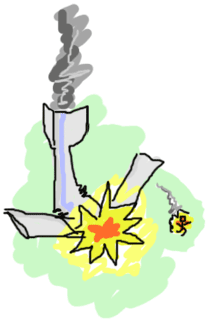
\includegraphics[width=1\linewidth]{letitcrash.png}
\end{wrapfigure}
Позже мы увидим как использовать эти инструменты, но сейчас я расскажу ещё об одном общем правиле Erlang: пусть процесс падает.
Но пусть он падает не как самолёт в авиакатастрофе с десятками человеческих жертв, а пусть падает как канатоходец, под которым натянута страховочная сеть.
Избегать ошибок, конечно же, нужно, но делать проверки на каждый тип ошибки в большинстве случаев нет необходимости.

Итак, Erlang умеет восстанавливаться после ошибок, организовывать код при помощи акторов, производить распределённое масштабирование и обеспечивать параллелизм.
Но это приводит нас к следующему разделу\ldots

\section{Не забывайтесь}
В книге будет много маленьких жёлто\--оранжевых разделов, с названиями похожими на это (их легко заметить).
Erlang в данный момент набирает популярность во многом благодаря пылким речам, которые могут ввести людей в заблуждение.
Могут убедить, что Erlang \--- нечто большее, чем есть на самом деле.
Эти напоминания помогут вам не забываться, если вы переполнены энтузиазмом сверх меры.

Первый случай такого заблуждения относится к мощным возможностям масштабирования, которые заложены в Erlang и осуществляются при помощи лёгких процессов.
Да, действительно, процессы в Erlang очень легки: единовременно могут существовать сотни тысяч таких процессов, но это не означает, что они должны существовать просто потому что есть такая возможность.
К примеру, вы создаёте игру\--стрелялку.
Было бы безумием представлять все объекты в игре, включая пули, при помощи акторов.
В такой игре вы сможете выстрелить только себе в ногу.
Пересылка сообщений от акторa к актору всё\--таки отнимает ресурсы, как бы малы они ни были.
Если будете дробить задачи слишком сильно, \emph{всё может сильно замедлиться}!

Я расскажу об этом подробнее, когда мы погрузимся в изучение достаточно глубоко, чтобы это нас начало беспокоить.
Но пока что имейте в виду, что бездумно использовать параллелизм при решении проблемы, совсем недостаточно, для того чтобы решение стало быстрым.
Не огорчайтесь!
Будут и случаи, когда использовать сотни процессов можно и нужно!
Просто не каждый случай \--- тот самый.

Ещё об Erlang говорят, что он может масштабироваться прямо пропорционально количеству вычислительных ядер, которые есть в вашем компьютере, но обычно это не так.
Возможность такая имеется, но большинство задач не получится запустить таким образом, чтобы всё исполнялось одновременно.
\begin{wrapfigure}{l}{0.3\linewidth}
    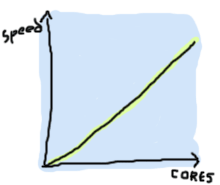
\includegraphics[width=1\linewidth]{scaling.png}
\end{wrapfigure}

Стоит помнить ещё об одном: хотя Erlang и делает некоторые вещи очень хорошо, всё\--таки технически возможно получить те же результаты при помощи других языков.
Верно также и обратное.
Тщательно оценивайте проблему и выбирайте правильный инструмент, исходя из той задачи, которую вы пытаетесь решить.
Erlang \--- не панацея и будет особенно плох в обработке изображений и сигналов или в качестве языка для написания драйверов.
Однако он будет блистать в области большого программного обеспечения для серверов (например: очереди, map\--reduce), в вычислениях совместно с другими языками, в высокоуровневой реализации протоколов и т.д.
Всё, что находится между этими полюсами, зависит лишь от вас.
Не обязательно ограничивать себя только серверными вычислениями на Erlang.
Были случаи, когда люди делали неожиданные и удивительные вещи.
Один из примеров это IANO \--- робот, созданный командой UNICT.
Они используют Erlang для реализации искусственного интеллекта и получили серебрянную медаль на соревновании eurobot в 2009 году.
Ещё один пример \--- Wings 3D.
Платформонезависимая программа трёхмерного моделирования (без рендерера) с открытым исходным кодом, которая написана на Erlang.

\section{Что нужно для изучения}
Для начала вам понадобится лишь текстовый редактор и среда Erlang.
Можно загрузить исходный код и сборки для Windows с официального сайта Erlang.
Не буду углубляться в детали установки, но для Windows достаточно скачать и запустить исполняемый файл.
Не забудьте добавить директорию Erlang в переменную окружения PATH, чтобы получить доступ к ней из командной строки.

В Debian\--подобных Linux дистрибутивах необходимо установить пакет командой \ops{\# apt-get install erlang}.
В Fedora (если установлен <<yum>>), можно проделать то же самое, набрав \ops{\# yum install erlang}.
Однако, официальные репозитории обычно содержат устаревшие версии пакетов Erlang.
Если вы будете использовать старую версию пакета, это может привести к расхождениям между вашим результатом и этим руководством.
К тому же, в определённых приложениях производительность будет снижена.
Поэтому я рекомендую вам компилировать всё из исходного кода.
Изучите содержимое файла README, который поставляется с пакетом, воспользуйтесь Google для получения подробностей установки, у них это получится намного лучше, чем у меня.

В FreeBSD существует много способов установки.
Если вы используете \ops{postmaster}, можно исполнить команду\\ 
\ops{postmaster lang/erlang}.\\ 
Для установки из портов вопользуйтесь командой\\ 
\ops{cd /usr/ports/lang/erlang;make install clean}.\\ 
В конце концов, если хотите воспользоваться пакетами, запустите\\  
\ops{pkg\_add -rv erlang}.\\ 
Если вы пользователь OSX, то можете установить Erlang командой\\ 
\ops{brew install erlang}\\ 
при помощи Homebrew или воспользуйтесь\\ 
\ops{port install erlang}, если предпочитаете MacPorts.\\ 
\colorbox{lgray}
{
\begin{minipage}{1.0\linewidth}
\textbf{Замечание:} на момент написания я использую Erlang версии R13B+, поэтому для наилучших результатов используйте такую же версию, либо более новую.
\end{minipage}
}
\section{Где искать помощь}
Есть несколько мест, где вам помогут.
Хорошую техническую документацию можно найти в man страницах, если вы используете Linux.
Например, в Erlang есть модуль lists (который мы скоро увидим): чтобы получить документацию по этому модулю напишите в консоли \ops{\$ erl -man lists}.

Инсталляция в Windows должна содержать документацию в формате HTML.
Её всегда можно скачать с \href{http://erlang.org/doc/}{официального сайта Erlang} или обратиться к одному из \href{http://erldocs.com}{альтернативных сайтов}.

Как только почувствуете, что пишете что\--то не то, обратитесь к правилам хорошего кодирования, которые можно найти \href{http://www.erlang.se/doc/programming_rules.shtml}{здесь}.
Код в этой книге будет стараться придерживаться этих правил.

Бывают случаи, когда простого понимания технических деталей недостаточно.
Когда наступает такой момент, я обращаюсь к двум источникам знаний: официальной \href{http://www.erlang.org/static/doc/mailinglist.html}{почтовой рассылке} (там есть чему поучиться) и irc каналу \#erlang на irc.freenode.net.

А если вы любите готовые рецепты, то \href{http://trapexit.org}{trapexit} это то что вам нужно.
Ещё они держат зеркало почтовой рассылки в виде форума и общую вики.
Там всегда можно найти что\--нибудь полезное.
